\documentclass[twocolumn]{article}
\usepackage[utf8]{inputenc}
\usepackage{graphicx}
\usepackage{tabularx}
\usepackage{subfigure}
\usepackage{hyperref}
\voffset = -100pt
\hoffset = -50pt
\headheight = 0pt
\textwidth = 550pt
\textheight = 750pt
\author{Name Surname }
\setlength{\columnsep}{0.3cm}
\usepackage{blindtext}
\pagestyle{empty}
\footskip = 0pt
\bibliographystyle{plain}
\usepackage{float}

\begin{document}

\section*{Viktor Pavlov 232211IAPM}
\section{Music Genre Classification via MFCC Analysis}
\begin{figure}[htbp]
  \centering
  \begin{minipage}[t]{0.5\columnwidth}
    \centering
    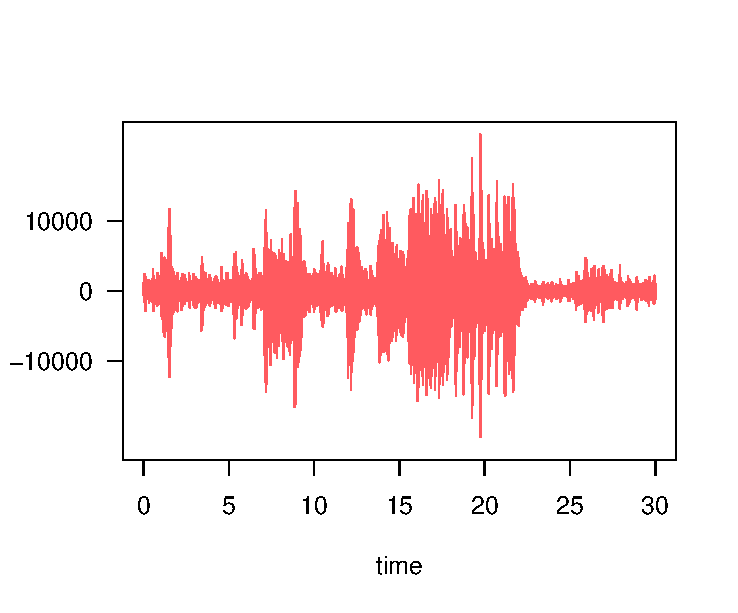
\includegraphics[width=\linewidth]{images/audio_jazz.pdf}
  \end{minipage}\hfill
  \begin{minipage}[t]{0.5\columnwidth}
    \centering
    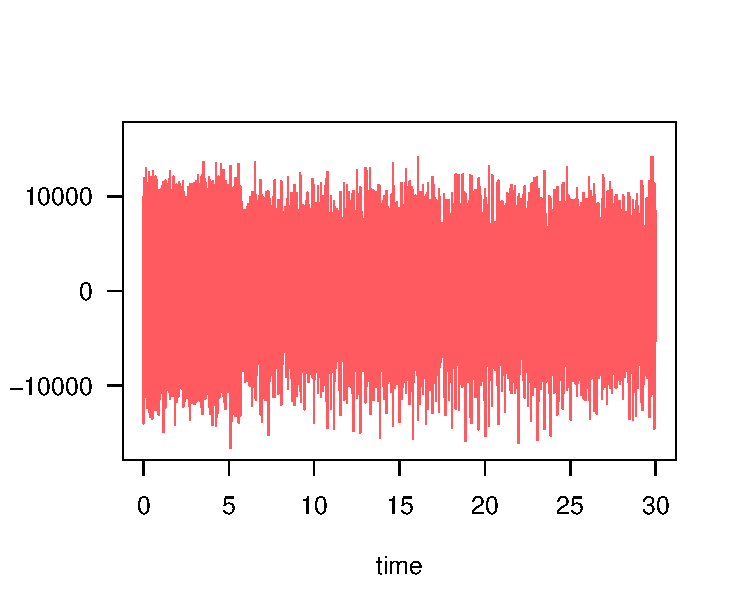
\includegraphics[width=\linewidth]{images/audio_metal.pdf}
  \end{minipage}
  \caption{Audio Waveforms of the files \texttt{jazz.00000.wav} (left) and \texttt{metal.00001.wav} (right).}
  \label{fig:waves}
\end{figure}
The goal of this project is to try music genre classification, utilizing audio feature extraction techniques together with clustering and classification data mining techniques. For this purpose, the GTZAN Genre Collection dataset~\cite{tzanetakis_essl_cook_2001} will be used. The dataset consists of $1000$ audio tracks, each $30$ seconds long. It contains $10$ genres, each represented by $100$ tracks. The tracks are all $22050$ Hz monophonic $16$-bit audio files in \texttt{.au} format. It's important to note, that this is a legacy dataset, collected from various sources, including personal CDs, radio and microphone recordings, with inconsistent quality~\cite{sturm2013gtzan}. Nevertheless, it's sufficient for our use case. Visualizations of audio signals from the dataset are displayed in Figure~\ref{fig:waves}.
\section{MFCC Audio Feature Extraction}
Mel-frequency cepstrum coefficients (MFCCs) convert complex audio signals into a compact spectral representation that highlights components critical to the human ear. Applications of MFCCs include speech recognition~\cite{ganchev2005comparative} and music genre classification~\cite{lerch2012introduction}. In particular, MFCCs can capture the timbral texture of audio, capturing subtle nuances, useful for distinguishing different musical styles. Various literature suggests that the first $12$ coefficients are sufficient for speech recognition, while it's recommended to use $20-40$ coefficients for musical audio signals. The precise number of coefficients can be determined by means of experimentation, and in context of this project, the first $30$ coefficients were used. The \texttt{tuneR} package~\cite{tuneR} was utilized for extracting the MFCCs. Visualization of MFCCs is displayed in Figure~\ref{fig:mfcc}.
\section{K-Means Clustering}
\begin{figure}[hht]
\centering
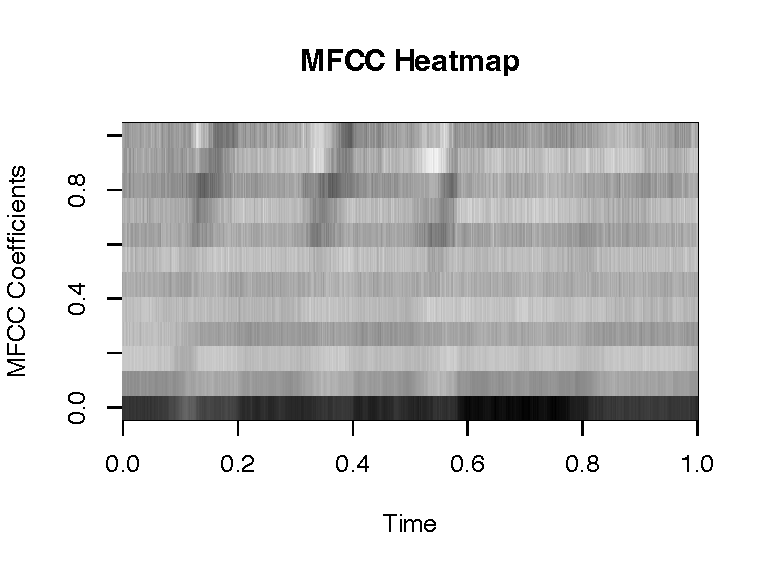
\includegraphics[width=0.49\textwidth]{images/mfcc_heatmap_8.pdf}
\caption{MFCC heatmap of the file \texttt{classical.00015.wav}.}
\label{fig:mfcc}
\end{figure}
While clustering all $10$ genres by MFCC features produced adequate results at first sight, only two genres were picked for simplification purposes. Results are displayed in Table~\ref{table:clustering_results}. Additionally, silhouette coefficient plot of the Pop and Metal genres clustering results is displayed in Figure~\ref{fig:corr}.
\begin{table}[H]
\centering
\begin{tabular}{lcc}
  \hline
 \textbf{Genre Pair} & \textbf{Cluster Sizes} & \textbf{Variance Ratio (\%)} \\
  \hline
 Pop vs Metal & 106, 94 & 46.8 \\
 Jazz vs Rock & 84, 116 & 34.3 \\
 Reggae vs Classical & 95, 104 & 26.1 \\
 Country vs Disco & 104, 96 & 40.9 \\
  \hline
\end{tabular}
\caption{K-Means Clustering Results for Different Genre Pairs.}
\label{table:clustering_results}
\end{table}
\section{Classification using Support Vector Machines (SVM)}
\begin{figure}[hht]
	\centering
	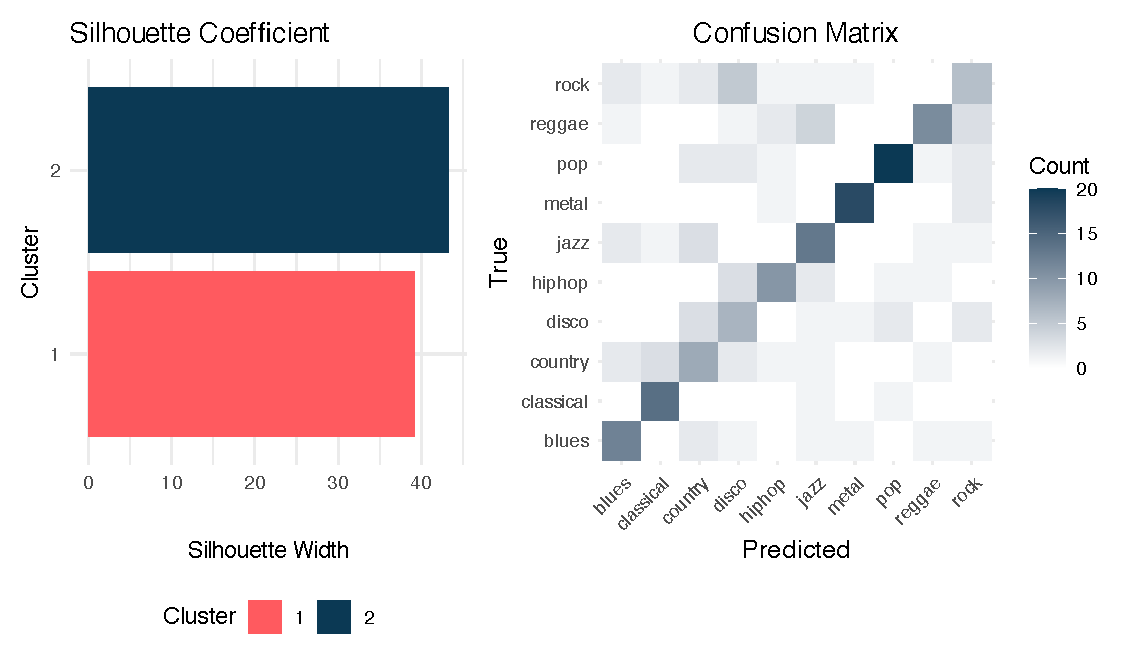
\includegraphics[width=0.49\textwidth]{images/clust_class.pdf}
  \caption{Pop vs Metal silhouette plot (left), Confusion matrix for all genres (right).}
	\label{fig:corr}
\end{figure}
For the classification task SVM classifier was utilized with the \textit{radial} kernel, yielding a $0.604$ accuracy. This result represents the optimal outcome obtained after experimenting with various numbers of MFCC coefficients. The model can potentially be improved by adding features like the spectral centroid and zero crossing rate, that capture nuances related to dynamics and tonality of the given audio sample. The \texttt{seewave} package~\cite{seewave} can be utilized for extraction of these additional features.
\bibliography{bibliography}
\end{document}
